\documentclass{article}
\usepackage{graphicx} 
\usepackage{multirow}
\usepackage{enumitem}
\usepackage{amssymb}
\usepackage{amsmath}
\usepackage{xcolor}
\usepackage{cancel}
\usepackage{tcolorbox}
\usepackage{geometry}
\usepackage{tikz}
\usepackage{tikz-3dplot}
\usepackage{pgfplots, tkz-euclide,calc}
    \usetikzlibrary{patterns,snakes,shapes.arrows,3d}
    \usepgfplotslibrary{fillbetween}
	\geometry{
		total = {160mm, 237mm},
		left = 25mm,
		right = 35mm,
		top = 30mm,
		bottom = 30mm,
	}

\newcommand{\jawab}{\textbf{Jawab}:}
\newcommand{\del}{\partial}
\begin{document}
    \pagenumbering{gobble}
    \begin{tabular}{|lcl|}
     \hline
     Nama&:&Teosofi Hidayah Agung\\
     NRP&:&5002221132\\
     \hline
    \end{tabular}
    \begin{enumerate}
        \item Tunjukkan bahwa:
        \begin{enumerate}
            \item $\nabla \times \left(r^2~\bar{r}\right) = 0$\\
            \jawab
            \begin{flalign*}
                \nabla \times \left(r^2~\bar{r}\right)&=\nabla \times \left(r^2~x\vec{i}+r^2~y\vec{j}+r^2~z\vec{k}\right)&\\
                &=\begin{vmatrix}
                    \vec{i}&\vec{j}&\vec{k}\\
                    \dfrac{\del}{\del x}&\dfrac{\del}{\del y}&\dfrac{\del}{\del z}\\
                    r^2x&r^2y&r^2z
                \end{vmatrix}&\\
                &=\left(\frac{\del}{\del y}(r^2z)-\frac{\del}{\del z}(r^2y)\right)\vec{i}-\left(\frac{\del}{\del x}(r^2z)-\frac{\del}{\del z}(r^2x)\right)\vec{j}+\left(\frac{\del}{\del x}(r^2y)-\frac{\del}{\del y}(r^2x)\right)\vec{k}&\\
                &=\left(0-0\right)\vec{i}-\left(0-0\right)\vec{j}+\left(0-0\right)\vec{k}&\\
                &=0\vec{i}+0\vec{j}+0\vec{k}&\\
                &=0\,\blacksquare
            \end{flalign*}
            
            \item $\nabla \cdot \bar{r}\,f(r) = 3f(r) + |r|\,\dfrac{df}{dr}$\\
            \jawab
            \begin{flalign*}
                \nabla r\,f(r)&=(\nabla r)f(r)+r(\nabla f(r))&\\
                &=3f(r)+r\left(\frac{\del f}{\del x}\vec{i}+\frac{\del f}{\del y}\vec{j}+\frac{\del f}{\del z}\vec{k}\right)&\\
                &=3f(r)+r\left(\frac{\del f}{\del r}\frac{\del r}{\del x}\vec{i}+\frac{\del f}{\del r}\frac{\del r}{\del y}\vec{j}+\frac{\del f}{\del r}\frac{\del r}{\del z}\vec{k}\right)&\\
                &=3f(r)+r\left(\frac{\del r}{\del x}\vec{i}+\frac{\del r}{\del y}\vec{j}+\frac{\del r}{\del z}\vec{k}\right)\frac{\del f}{\del r}&\\
                &=3f(r)+r\left(\nabla r\right)\frac{\del f}{\del r}&\\
                &=3f(r)+r\left(\frac{r}{r}\right)\frac{\del f}{\del r}&\\
                &=3f(r)+|r|\frac{df}{dr}\,\blacksquare
            \end{flalign*}
        \end{enumerate}

        \item Diberikan integral berikut $\displaystyle \oint_{C}(2xy-x^2)dx+(x+y^2)dy$ jika $C$ 
        adalah kurva tertutup yang dibatasi oleh $y=x^2$, dan $8x=y^2$.
        \begin{enumerate}
            \item Hitung integral tersebut dengan menggunakan teorema Green.\\
            \jawab\\
            Daerah $D$ yang dibatasi kurva $C$ adalah sebagai berikut:
            \begin{center}
                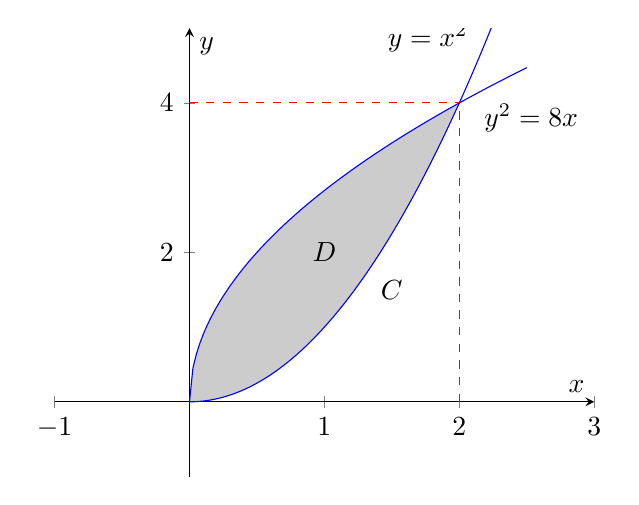
\begin{tikzpicture}
                    \begin{axis}[
                        axis lines = center,
                        xlabel = $x$,
                        ylabel = $y$,
                        xmin = -1, xmax = 3,
                        ymin = -1, ymax = 5,
                    ]
                    \addplot [
                        label=$y=x^2$,
                        name path=A,
                        domain=0:2.5, 
                        samples=100, 
                        color=blue,
                    ]
                    {x^2} node[pos=0.75](endofplotsquare){} ;
                    \node [above left] at (endofplotsquare) {$y=x^2$};
                    \addplot [
                        name path=B,
                        domain=0:2.5, 
                        samples=100, 
                        color=blue,
                    ]
                    {sqrt(8*x)} node[pos=0.9](endofplotsquare){} ;
                    \addplot [
                        dashed,
                        domain=0:2, 
                        samples=10, 
                        color=red,
                    ]
                    {4};
                    \addplot[dashed, 
                    samples=10, smooth,domain=1:3,red] coordinates {(2,0)(2,4)};
                    \node [below right] at (endofplotsquare) {$y^2=8x$};
                    \addplot[fill=gray,opacity=0.4] fill between[of=A and B,split,soft clip={domain=0:2}];
                    \node at (axis cs:1,2) {$D$};
                    \node at (axis cs:1.5,1.5) {$C$};
                    \end{axis}
                \end{tikzpicture}
            \end{center}
            Sehingga nilai integralnya dengan menggunakan teorema Green adalah
            \begin{flalign*}
                \oint_{C}(2xy-x^2)dx+(x+y^2)dy&=\iint_{D}\left(\frac{\del}{\del x}(x+y^2)-\frac{\del}{\del y}(2xy-x^2)\right)dA&\\
                &=\iint_{D}(1-2x)dA&\\
                &=\int_{0}^{2}\int_{2\sqrt{2}\sqrt{x}}^{x^2}(1-2x)dydx&\\
                &=\int_{0}^{2}\left[y-2xy\right]_{2\sqrt{2}\sqrt{x}}^{x^2}dx&\\
                &=\int_{0}^{2}\left[x^2-2x(x^2)-2\sqrt{2}\sqrt{x}+4x\sqrt{2}\sqrt{x}\right]dx&\\
                &=\int_{0}^{2}\left[x^2-2x^3-2\sqrt{2}\sqrt{x}+4\sqrt{2}x\sqrt{x}\right]dx&\\
                &=\int_{0}^{2}\left[x^2-2x^3-2\sqrt{2}\sqrt{x}+4\sqrt{2}x^{3/2}\right]dx&\\
                &=\left[\frac{x^3}{3}-\frac{x^4}{2}-\frac{4\sqrt{2}}{3}x^{3/2}+\frac{8\sqrt{2}}{5}x^{5/2}\right]_{0}^{2}&\\
                &=\frac{8}{3}-8-\frac{16}{3}+\frac{64}{5}&\\
                &=\frac{32}{15}
            \end{flalign*}
            \item Hitung integral tersebut secara langsung tanpa menggunakan teorema Green.\\
            \jawab\\
            Misalkan $C_1$ adalah kurva $y=x^2$ dan $C_2$ adalah kurva $8x=y^2$.
            \begin{enumerate}[label=(\roman*)]
                \item Hitung integral di sepanjang $C_1$.
                \begin{flalign*}
                    \int_{C_1}(2xy-x^2)dx+(x+y^2)dy&=\int_{0}^{2}\left(2x(x^2)-x^2\right)dx+\left(x+x^2\right)2xdx&\\
                    &=\int_{0}^{2}\left(2x^3-x^2+x+2x^2\right)dx&\\
                    &=\int_{0}^{2}\left(2x^3+x^2+x\right)dx&\\
                    &=\left[\frac{1}{2}x^4+\frac{1}{3}x^3+\frac{1}{2}x^2\right]_{0}^{2}&\\
                    &=\frac{1}{2}(16)+\frac{1}{3}(8)+\frac{1}{2}(4)&\\
                    &=8+\frac{8}{3}+2&\\
                    &=\frac{32}{3}
                \end{flalign*}
                \item Hitung integral di sepanjang $C_2$.
                \begin{flalign*}
                    \int_{C_2}(2xy-x^2)dx+(x+y^2)dy&=\int_{0}^{4}\left(2\left(\frac{y^2}{8}\right)y-\left(\frac{y^2}{8}\right)^2\right)\frac{y}{4}dy+\left(\left(\frac{y^2}{8}\right)+y^2\right)dy&\\
                    &=\int_{0}^{4}\left(\frac{y^4}{16}-\frac{y^5}{256}+\frac{y^3}{8}+y^2\right)dy&\\
                    &=\left[\frac{1}{5}\frac{y^5}{16}-\frac{1}{6}\frac{y^6}{256}\right]_{0}^{4}+\left[\frac{1}{4}\frac{y^4}{8}+\frac{1}{3}y^3\right]_{0}^{4}&\\
                    &=\frac{1}{5}\frac{4^5}{16}-\frac{1}{6}\frac{4^6}{256}+\frac{1}{4}\frac{4^4}{8}+\frac{1}{3}4^3&\\
                    &=\frac{592}{15}
                \end{flalign*}
            \end{enumerate}
            Sehingga nilai integralnya adalah
            \begin{flalign*}
                \oint_{C}(2xy-x^2)dx+(x+y^2)dy&=\oint_{C_2-C1}(2xy-x^2)dx+(x+y^2)dy=&\\
                &=\frac{592}{15}-\frac{32}{3}&\\
                &=\frac{32}{15}
            \end{flalign*}
        \end{enumerate}
        \item Diberikan vektor gaya $\bar{A}=(2xy+z)\vec{i}+y^2\vec{j}+(x+3y)\vec{k}$ dan $S$ 
        adalah permukaan yang dibatasi oleh $z=4-y^2,\,x=0,\,x=2$ dan bidang $xy$.
        \begin{enumerate}
            \item Gambarkan geometri batasan permukaan benda.\\
            \jawab
            \begin{center}
                \tdplotsetmaincoords{60}{110}
                \begin{tikzpicture}[tdplot_main_coords,scale=0.85]
                    \pgfmathsetmacro{\step}{0.01}
                    %%% Coordinate axis
                    \draw[thick,->] (0,0,0) -- (3,0,0) node [below left] {\footnotesize$x$};
                    \draw[dashed] (0,0,0) -- (-3,0,0);
                    \draw[thick,->] (0,0,0) -- (0,3,0) node [right] {\footnotesize$y$};
                    \draw[dashed] (0,0,0) -- (0,-3,0);
                    \draw[thick] (0,0,0.0) -- (0,0,4.0);
                    % Region of integration
		            \draw[gray,thick,fill=yellow,opacity=0.35] (2,2,0) -- (2,-2,0) -- (-2,-2,0) -- (-2,0,0) -- cycle;
                    % The surface
                    \foreach \x in {0,\step,...,2.0}{
                        \draw[cyan,thick,opacity=0.25] plot[domain=-2:2,smooth,variable=\t] ({\x},{\t},{4.0 - \t*\t}); 
                    }
                    %negative surface
                    \foreach \x in {0,\step,...,2.0}{
                        \draw[cyan,thick,opacity=0.25] plot[domain=-2:2,smooth,variable=\t] ({-\x},{\t},{4.0 - \t*\t}); 
                    }
                    % The curves slicing the surface
                    \draw[blue,thick,opacity=0.5] plot[domain=-2:2,smooth,variable=\t] ({-2.0},{\t},{4.0 - \t*\t});
                    \draw[blue,thick,opacity=0.5] plot[domain=-2:2,smooth,variable=\t] ({2.0},{\t},{4.0 - \t*\t});
                    %
                    \node[blue,above right] at (0,2.5,4.125) {$z = 4 - y^2$};
                    % Last part of the z axis
                    \draw[thick,->] (0,0,4.0) -- (0,0,5.0) node [above] {\footnotesize$z$};	
                    % line boundary
                    \draw[red,dashed] (2,-2,0) -- (2,2,0);
                    \draw[red,dashed] (-2,-2,0) -- (-2,2,0);
                    \draw[red,dashed] (2,2,0) -- (-2,2,0);
                    \draw[red,dashed] (-2,2,0) -- (2,2,0);
                    \foreach \x in {-2,2} 
                        \draw[shift={(\x,0,0)},color=black] (0pt,0.1pt,0pt) -- (0pt,-0.1pt,0pt) node[below] {$\x$};
                    \foreach \x in {-2,2} 
                        \draw[shift={(0,\x,0)},color=black] (0.1pt,0pt,0pt) -- (-0.1pt,0pt,0pt) node[below] {$\x$};
                    %point
                    \node[cyan,right] at (0,2,3.5) {$S$};
                    \node[red,right] at (1,-1,0) {$D$};
                \end{tikzpicture}
                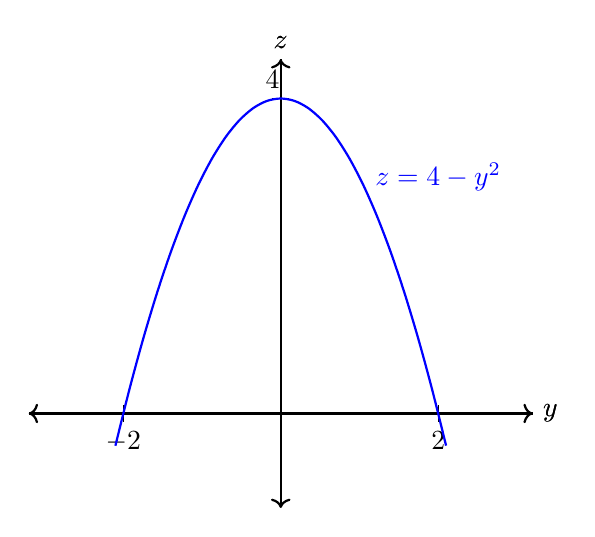
\begin{tikzpicture}
                    \draw[thick,->] (-3.2,0) -- (3.2,0) node[right] {$y$};
                    \draw[thick,->] (0,-1.0) -- (0,4.5) node[above] {$z$};
                    \draw[thick,<-] (-3.2,0) -- (3.2,0) node[right] {$y$};
                    \draw[thick,<-] (0,-1.2) -- (0,4.5) node[above] {$z$};
                    
                    \foreach \x in {-2,2} \draw[shift={(\x,0)},color=black] (0pt,3pt) -- (0pt,-3pt) node[below] {$\x$};
                    \draw [shift={(0,4)},color=black] (3pt,0pt) -- (-3pt,0pt) node[above] {$4$};
                    
                    \draw[thick,blue,domain=-2.1:2.1,smooth] plot (\x,{4-(\x)^2}) {};
                    \node[blue] at (2,3) {$z=4-y^2$};
                \end{tikzpicture}
            \end{center}
            \item Hitunglah $\displaystyle \iint_S \bar{A}\cdot\bar{n}\,dS$ dengan menggunakan 
            teorema Gauss.\\
            \jawab
            \begin{flalign*}
                \iint_S \bar{A}\cdot\bar{n}\,dS&=\iiint_V \nabla\cdot\bar{A}\,dV&\\
                &=\iiint_V \left(\frac{\del}{\del x}(2xy+z)+\frac{\del}{\del y}(y^2)+\frac{\del}{\del z}(x+3y)\right)dV&\\
                &=\iiint_V (2y+2y+0)dV&\\
                &=\int_{0}^{2}\int_{0}^{2}\int_{0}^{4-y^2} 4y\,dz\,dy\,dx&\\
                &=\int_{0}^{2}\int_{0}^{2} 4y(4-y^2)dy\,dx&\\
                &=\int_{0}^{2}\int_{0}^{2} 16y-4y^3\,dy\,dx&\\
                &=\int_{0}^{2} \left[8y^2-y^4\right]_{0}^{2}dx&\\
                &=\int_{0}^{2} \left[8(2)^2-(2)^4\right]dx&\\
                &=\int_{0}^{2} \left[8(4)-16\right]dx&\\
                &=\int_{0}^{2} 16\,dx=32
            \end{flalign*}
            \item Hitunglah $\displaystyle \iint_S \bar{A}\cdot\bar{n}\,dS$ secara langsung 
            tanpa menggunakan teorema Gauss.\\
            \jawab\\
            Diketahui $g(x,y,z)=4-y^2$ dan misalkan $D$ adalah daerah yang berada dibawah permukaan.
            \begin{flalign*}
                \iint_S \bar{A}\cdot\bar{n}\,dS&=\iint_D \left(-Pg_x-Qg_y+R\right)\,dS&\\
                &=\iint_D \left(-(2xy+z)0-y^2(-2y)+(x+3y)0\right)\,dS&\\
                &=\iint_D 2y^3\,dS&\\
                &=\int_{0}^{2}\int_{0}^{2} 2y^3\,dy\,dx&\\
                &=\int_{0}^{2} \left[\frac{1}{2}y^4\right]_{0}^{2}dx&\\
                &=\int_{0}^{2} \left[\frac{1}{2}(2)^4\right]dx&\\
                &=\int_{0}^{2} 8\,dx=16
            \end{flalign*}
            
        \end{enumerate}
    \end{enumerate}
\end{document}